\subsubsection{The 2D cylindrical shell benchmarks by Davies et al.}
\label{sec:benchmark-2D_cylindrical_shell}

\textit{This section was contributed by William Durkin and Wolfgang Bangerth.}

All of the benchmarks presented so far take place in a Cartesian domain.
Davies et al.~describe a benchmark (in a paper that is currently still being
written) for a 2D spherical Earth that is
nondimensionalized such that
\begin{table*}[h]
 \centering
 \begin{tabular}{ l l }
    $r_{\min}$ = 1.22 &  $\left. T \right|_{r_{min}}$ = 1 \\
    $r_{\max}$ = 2.22 &  $\left. T \right|_{r_{max}}$ = 0
 \end{tabular}
\end{table*}

The benchmark is run for a series of approximations (Boussinesq, Extended Boussinesq,
Truncated Anelastic Liquid, and Anelastic Liquid), and temperature, velocity, and heat flux
calculations are compared with the results of other mantle modeling programs. \aspect{}
will output all of these values directly except for the Nusselt number, which
we must calculate ourselves from the heat fluxes that \aspect{} can compute.
The Nusselt number of the top and bottom surfaces, ${Nu}_T$ and ${Nu}_B$,
respectively, are defined by the authors of the benchmarks as
\begin{equation}
\label{eq:davies-NuTop}
{Nu}_{T} = \frac{\ln(f)}{2{\pi}r_{\max}(1-f)}\int \limits_{0}^{2\pi} \frac{\partial T}{\partial r}\, \text{d}\theta  \\
\end{equation}
and
\begin{equation*}
\label{eq:davies-NuBottom}
{Nu}_{B} = \frac{f \ln(f)}{2{\pi}r_{\min}(1-f)}\int \limits_{0}^{2\pi} \frac{\partial T}{\partial r}\, \text{d}\theta \\
\end{equation*}
where $f$ is the ratio $\frac{r_{\min}}{r_{\max}}$.

We can put this in terms of heat flux
\begin{equation*}
  q_r = -k\frac{\partial T}{\partial r}
\end{equation*}
through the inner and outer surfaces,
where $q_r$ is heat flux in the radial direction. Let $Q$ be the total heat that flows through a surface,
\begin{equation*}
  Q = \int \limits_{0}^{2\pi} q_r\, \text{d}\theta,
\end{equation*}
then \eqref{eq:davies-NuTop} becomes
\begin{equation*}
  {Nu}_{T} = \frac{-Q_{T}\ln(f)}{2\pi{r_{\max}}(1-f)k}
\end{equation*}
and similarly
\begin{equation*}
  {Nu}_{B} = \frac{-Q_{B}f\ln(f)}{2\pi{r_{\min}}(1-f)k}.
\end{equation*}
$Q_T$ and $Q_B$ are heat fluxes that \aspect{} can readily compute through the
\texttt{heat flux statistics} postprocessor (see
Section~\ref{parameters:Postprocess/List of postprocessors}).
For further details on the nondimensionalization and equations used for each
approximation, refer to Davies et al.

The series of benchmarks is then defined by a number of cases relating to the
exact equations chosen to model the fluid. We will discuss these in the
following.


\paragraph{Case 1.1: BA\_Ra104\_Iso\_ZS.}
\label{sec:davies-case11_BA}

This case is run with the following settings:
\begin{itemize}
\item Boussinesq Approximation
\item Boundary Condition: Zero-Slip
\item Rayleigh Number = $10^4$
\item Initial Conditions: $D = 0, O = 4$
\item $\eta(T) = 1$
\end{itemize}
where $D$ and $O$ refer to the degree and order of a spherical harmonic that describes the
initial temperature. While the initial conditions matter, what is important
here though is that the system evolve to four convective cells since we are
only interested in the long term, steady state behavior.

The model is relatively straightforward to set up, basing the input file on
that discussed in Section~\ref{sec:shell-simple-2d}. The full input file can
be found at \url{benchmarks/davies_et_al/case-1.1.prm}, with the interesting
parts excerpted as follows:

\lstinputlisting[language=prmfile]{cookbooks/benchmarks/davies_et_al/doc/case-1.1.prm.out}

We use the same trick here as in Section~\ref{sec:cookbooks-simple-box} to
produce a model in which the density $\rho(T)$ in the temperature equation
\eqref{eq:temperature} is almost constant (namely, by choosing a very small
thermal expansion coefficient) as required by the benchmark, and instead
prescribe the desired Rayleigh number by choosing a correspondingly large
gravity.

Results for this and the other cases are shown below.


\paragraph{Case 2.1: BA\_Ra104\_Iso\_FS.}
\label{sec:davies-case21_BA}

Case 2.1 uses the following setup, differing only in the boundary conditions:
\begin{itemize}
\item Boussinesq Approximation
\item Boundary Condition: Free-Slip
\item Rayleigh Number = $10^4$
\item Initial Conditions: $D = 0, O = 4$
\item $\eta(T) = 1$
\end{itemize}

As a consequence of the free slip boundary conditions, any solid body rotation
of the entire system satisfies the Stokes equations with their boundary
conditions. In other words, the solution of the problem is not unique: given a
solution, adding a solid body rotation yields another solution. We select
arbitrarily the one that has no net rotation (see
Section~\ref{parameters:Nullspace_20removal}). The section in the input file
that is relevant is then as follows (the full input file resides at
\url{benchmarks/davies_et_al/case-2.1.prm}):
\index[prmindex]{Remove nullspace}
\index[prmindexfull]{Nullspace removal!Remove nullspace}

\lstinputlisting[language=prmfile]{cookbooks/benchmarks/davies_et_al/doc/case-2.1.prm.out}

Again, results are shown below.


\paragraph{Case 2.2: BA\_Ra105\_Iso\_FS.}
\label{sec:davies-case22_BA}

Case 2.2 is described as follows:
\begin{itemize}
\item Boussinesq Approximation
\item Boundary Condition: Free-Slip
\item Rayleigh Number = $10^5$
\item Initial Conditions: Final conditions of case 2.1 (BA\_Ra104\_Iso\_FS)
\item $\eta(T) = 1$
\end{itemize}
In other words, we have an increased Rayleigh number and begin with the final
steady state of case 2.1. To start the model where case 2.1 left off, the
input file of case 2.1, \url{benchmarks/davies_et_al/case-2.1.prm}, instructs
\aspect{} to checkpoint itself every few time steps (see
Section~\ref{sec:checkpoint-restart}). If case 2.2 uses the same
output directory, we can then resume the computations from this checkpoint with
an input file that prescribes a different Rayleigh number and a later input time:

\lstinputlisting[language=prmfile]{cookbooks/benchmarks/davies_et_al/doc/case-2.2.prm.out}

We increase the Rayleigh number to $10^5$ by increasing the magnitude of
gravity in the input file.  The full script for case 2.2 is located in
\url{benchmarks/davies_et_al/case-2.2.prm}


\paragraph{Case 2.3: BA\_Ra103\_vv\_FS.}
\label{sec:davies-case23_BA}

Case 2.3 is a variation on the previous one:
\begin{itemize}
\item Boussinesq Approximation
\item Boundary Condition: Free-Slip
\item Rayleigh Number = $10^3$
\item Initial Conditions: Final conditions of case 2.1 (BA\_Ra104\_Iso\_FS)
\item $\eta(T) = 1000^{-T}$
\end{itemize}
The Rayleigh number is smaller here (and is selected using the gravity
parameter in the input file, as before), but the more important change is that the
viscosity is now a function of temperature. At the time of writing, there is
no material model that would implement such a viscosity, so we
create a plugin that does so for us (see Sections~\ref{sec:extending} and
\ref{sec:write-plugin} in
general, and Section~\ref{sec:material-models} for material models in
particular). The code for it is located in
\url{benchmarks/davies_et_al/case-2.3-plugin/VoT.cc} (where ``VoT'' is short
for ``viscosity as a function of temperature'') and is essentially a copy of
the \texttt{simpler} material model. The primary change compared to the
\texttt{simpler} material model is the line about the viscosity in the
following function:
\begin{lstlisting}[frame=single,language=C++]
template <int dim>
void
VoT<dim>::
evaluate(const typename Interface<dim>::MaterialModelInputs &in,
         typename Interface<dim>::MaterialModelOutputs &out) const
{
  for (unsigned int i=0; i<in.position.size(); ++i)
    {
      out.viscosities[i] = eta*std::pow(1000,(-in.temperature[i]));
      out.densities[i] = reference_rho * (1.0 - thermal_alpha * (in.temperature[i] - reference_T));
      out.thermal_expansion_coefficients[i] = thermal_alpha;
      out.specific_heat[i] = reference_specific_heat;
      out.thermal_conductivities[i] = k_value;
      out.compressibilities[i] = 0.0;
    }
}
\end{lstlisting}
Using the method described in Sections~\ref{sec:benchmark-run} and
\ref{sec:write-plugin}, and the files in
the \texttt{benchmarks/davies\_et\_al/case-2.3-plugin}, we can compile our new
material model into a shared library that we can then reference from the input file.
The complete input file for case 2.3 is located in
\url{benchmarks/davies_et_al/case-2.3.prm} and contains among others the
following parts:

\lstinputlisting[language=prmfile]{cookbooks/benchmarks/davies_et_al/doc/case-2.3.prm.out}


\paragraph{Results.}

In the following, let us discuss some of the results of the benchmark setups
discussed above. First, the final steady state temperature fields are shown in
Fig.~\ref{fig:davies-2DcylinderFSS}. It is immediately obvious how the
different Rayleigh numbers affect the width of the plumes. If one imagines a
setup with constant gravity, constant inner and outer temperatures and
constant thermal expansion coefficient (this is not how we describe it in the
input files, but we could have done so and it is closer to how we intuit about
fluids than adjusting the gravity), then the Rayleigh number is inversely
proportional to the viscosity -- and it is immediately clear that larger
Rayleigh numbers (corresponding to lower viscosities) then lead to thinner
plumes. This is nicely reflected in the visualizations.

\begin{figure}[h]
  \subfigure[Case 1.1]{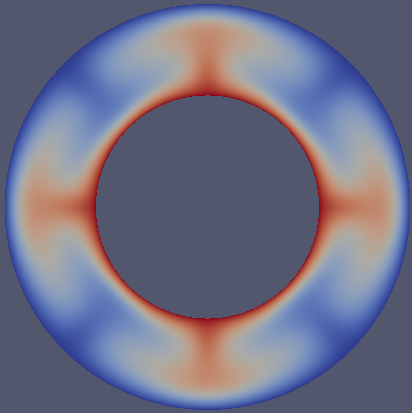
\includegraphics[width=0.23\textwidth]{cookbooks/benchmarks/davies_et_al/doc/case11_final.png}}
  \hfill
  \subfigure[Case 2.1]{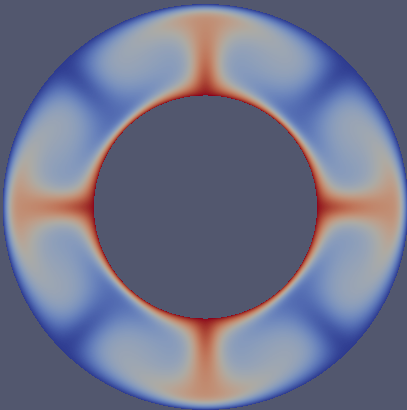
\includegraphics[width=0.23\textwidth]{cookbooks/benchmarks/davies_et_al/doc/case21_final.png}}
  \hfill
  \subfigure[Case 2.2]{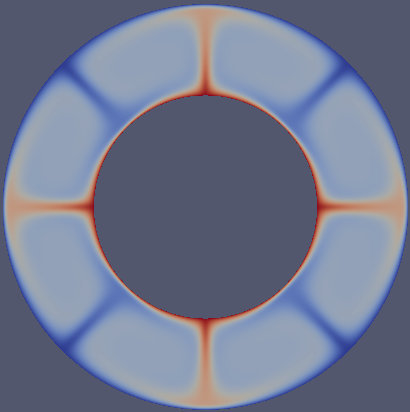
\includegraphics[width=0.23\textwidth]{cookbooks/benchmarks/davies_et_al/doc/case22_final.png}}
  \hfill
  \subfigure[Case 2.3]{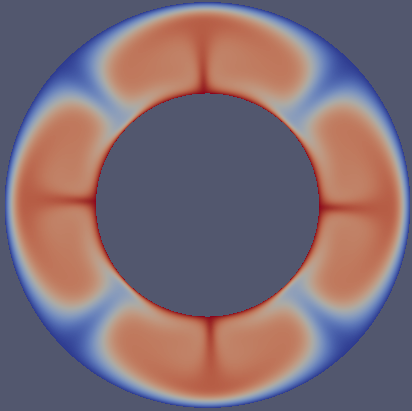
\includegraphics[width=0.23\textwidth]{cookbooks/benchmarks/davies_et_al/doc/case23_final.png}}
  \hfill
  \caption{\it Davies et al.~benchmarks: Final steady state temperature fields for
    the 2D cylindrical benchmark cases.}
  \label{fig:davies-2DcylinderFSS}
\end{figure}

Secondly, Fig.~\ref{fig:davies-2DcylinderVrms} shows the root mean square
velocity as a function of time for the various cases. It is obvious that they
all converge to steady state solutions. However, there is an initial transient
stage and, in cases 2.2 and 2.3, a sudden jolt to the system at the time where
we switch from the model used to compute up to time $t=2$ to the
different models used after that.

\begin{figure}[h]
  \subfigure[Case 1.1]{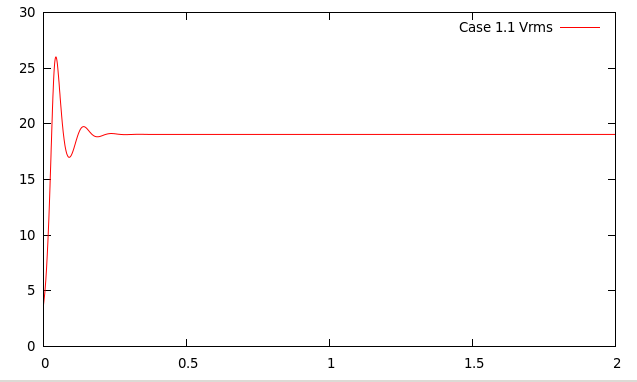
\includegraphics[width=0.48\textwidth]{cookbooks/benchmarks/davies_et_al/doc/Case11Vrms.png}}
  \hfill
  \subfigure[Case 2.1]{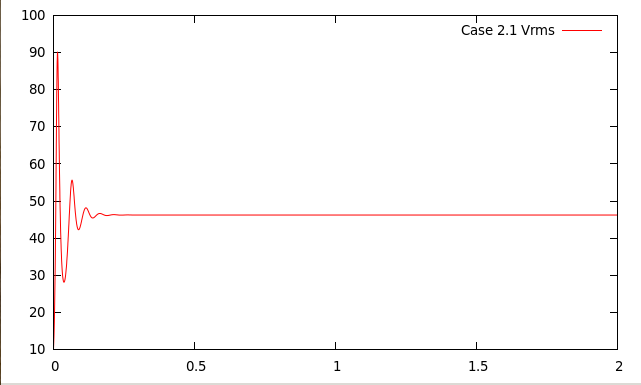
\includegraphics[width=0.48\textwidth]{cookbooks/benchmarks/davies_et_al/doc/Case21Vrms.png}}
  \\
  \subfigure[Case 2.2]{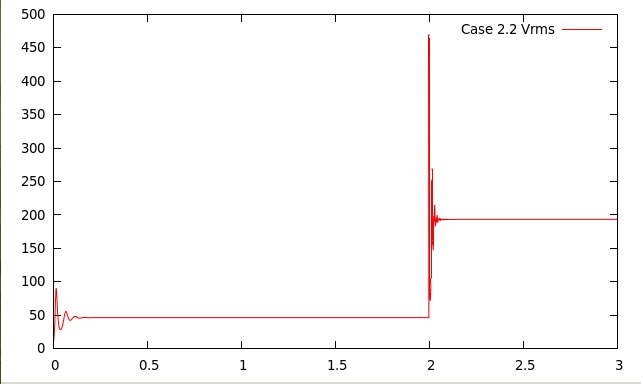
\includegraphics[width=0.48\textwidth]{cookbooks/benchmarks/davies_et_al/doc/Case22Vrms.png}}
  \hfill
  \subfigure[Case 2.3]{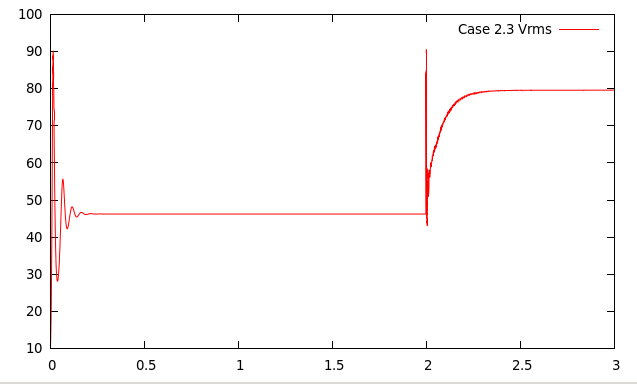
\includegraphics[width=0.48\textwidth]{cookbooks/benchmarks/davies_et_al/doc/Case23Vrms.png}}
  \hfill
  \caption{\it Davies et al.~benchmarks: $V_{\text{rms}}$ for 2D Cylindrical Cases. Large jumps occur when transitioning from case 2.1 to cases 2.2 and 2.3 due to the instantaneous change of parameter settings.}
  \label{fig:davies-2DcylinderVrms}
\end{figure}

These runs also produce quantitative data that will be published along with
the concise descriptions of the benchmarks and a comparison with other
codes. In particular, some of the criteria listed above to judge the accuracy
of results are listed in Table~\ref{tab:davies-et-al-results}.%
\footnote{The input files available in the \texttt{benchmarks/davies\_et\_al}
  directory use 5 global refinements in order to provide cases that can be run
  without excessive trouble on a normal computer. However, this is not enough
  to achieve reasonable accuracy and both the data shown below and the data
  submitted to the benchmarking effort uses 7
  global refinement steps, corresponding to a mesh with 1536 cells in
  tangential and 128 cells in radial direction. Computing on such meshes is
  not cheap, as it leads to a problem size of more than 2.5 million
  unknowns. It is best done using a parallel computation.}

\begin{table}[tbp]
  \centering
  \begin{tabular}{|l|c|c|c|c|}
    \hline
    Case & $\left<T\right>$ & $Nu_T$ & $Nu_B$ & $V_{\text{rms}}$
    \\ \hline
    1.1 & 0.403 & 2.464 & 2.468 & 19.053
    \\
    2.1 & 0.382 & 4.7000 & 4.706 & 46.244
    \\
    2.2 & 0.382 & 9.548 & 9.584 & 193.371
    \\
    2.3 & 0.582 & 5.102 & 5.121 & 79.632
    \\ \hline
  \end{tabular}
  \caption{\it Davies et al. benchmarks: Numerical results for some of the output quantities required by the benchmarks and the various cases considered.}
  \label{tab:davies-et-al-results}
\end{table}
